\documentclass[border=10pt]{standalone}
\usepackage{tikz}
\usetikzlibrary{calc, positioning}

\begin{document}

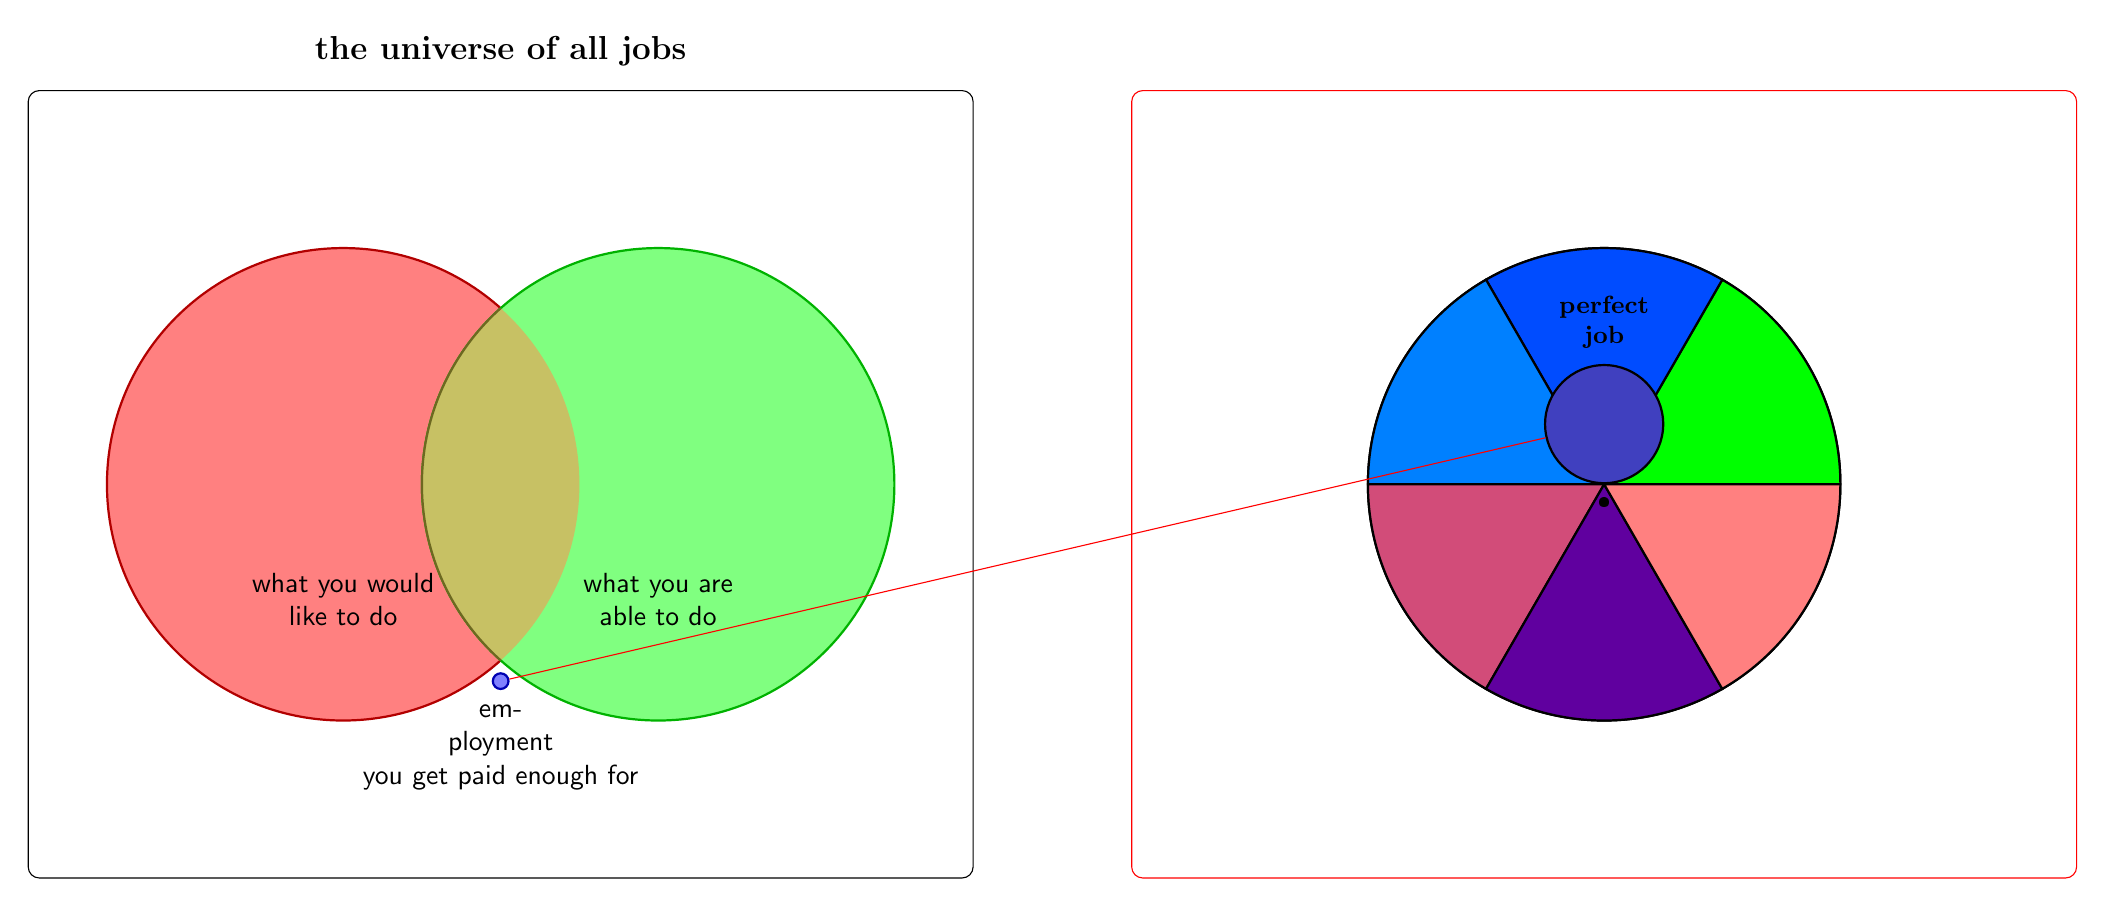
\begin{tikzpicture}[
    font=\sffamily,
    every node/.style={align=center},
    box/.style={draw, rectangle, rounded corners, inner sep=10pt, minimum width=12cm, minimum height=10cm},
    circle1/.style={fill=red!50, draw=red!70!black, thick},
    circle2/.style={fill=green!50, draw=green!70!black, thick},
    intersection/.style={fill=olive!50, draw=olive!70!black, thick},
    employment/.style={fill=blue!50, draw=blue!70!black, thick, circle, inner sep=2pt},
    perfectjob/.style={fill=blue!50!gray, draw=black, thick, circle, inner sep=0pt, minimum size=1.5cm},
    segment/.style={draw=black, thick, fill=#1},
    label/.style={font=\small, text=black}
]

% Left panel: Universe of all jobs
\node[box] (leftbox) at (0,0) {};
\node[above=5pt of leftbox.north, font=\large\bfseries] {the universe of all jobs};

% Circles
\draw[circle1] (-2,0) circle (3cm) node[below=1cm, text width=3cm] {what you would like to do};
\draw[circle2] (2,0) circle (3cm) node[below=1cm, text width=3cm] {what you are able to do};

% Intersection
\begin{scope}
    \clip (-2,0) circle (3cm);
    \fill[intersection] (2,0) circle (3cm);
\end{scope}

% Employment dot
\node[employment] (employment) at (0,-2.5) {};
\node[below=2pt of employment, text width=4cm, align=center] {em-\\ployment\\you get paid enough for};

% Right panel: Perfect job diagram
\node[box, draw=red, right=2cm of leftbox] (rightbox) {};
\coordinate (center) at (rightbox.center);

% Draw the circle and segments
\draw[thick, black] (center) circle (3cm);

% Segments (6 parts)
\foreach \angle/\color in {0/green, 60/blue!70!cyan, 120/blue!50!cyan, 180/purple!70, 240/purple!50!blue, 300/red!50} {
    \fill[segment=\color] (center) -- ++(\angle:3cm) arc (\angle:\angle+60:3cm) -- cycle;
}

% Perfect job label
\node[perfectjob, anchor=south] (perfectjob) at (center) {};
\node[above=2pt of perfectjob, font=\small\bfseries] {perfect\\job};
\node[below=1pt of perfectjob] {\textbullet};

% Red connecting line
\draw[red, thin] (employment) -- (perfectjob);

\end{tikzpicture}

\end{document}